% coding:utf-8

%----------------------------------------
%FOSAEBV, a LaTeX-Code for a summary of realtime image processing
%Copyright (C) 2013, Mario Felder

%This program is free software; you can redistribute it and/or
%modify it under the terms of the GNU General Public License
%as published by the Free Software Foundation; either version 2
%of the License, or (at your option) any later version.

%This program is distributed in the hope that it will be useful,
%but WITHOUT ANY WARRANTY; without even the implied warranty of
%MERCHANTABILITY or FITNESS FOR A PARTICULAR PURPOSE.  See the
%GNU General Public License for more details.
%----------------------------------------

\documentclass[a5paper,10pt,fleqn]{book}

\usepackage{fosaebv_layout}

%\setboolean{ti}{true}        % Anleitung für TI-89

\title{Formelsammlung Echtzeit Bildverarbeitung}
% \ifti
% \title{Formelsammlung Physik \\ Mit Anleitung zu TI-89}
% \fi

\author{Mario Felder}
\date{\today}

%\catcode `\*=\active
%\def *{\cdot}

\begin{document}

\maketitle
\thispagestyle{empty}
\cleardoublepage
\pagenumbering{Roman}
\tableofcontents

% coding:utf-8

%----------------------------------------
%FOSAEBV, a LaTeX-Code for a summary of realtime image processing
%Copyright (C) 2013, Mario Felder

%This program is free software; you can redistribute it and/or
%modify it under the terms of the GNU General Public License
%as published by the Free Software Foundation; either version 2
%of the License, or (at your option) any later version.

%This program is distributed in the hope that it will be useful,
%but WITHOUT ANY WARRANTY; without even the implied warranty of
%MERCHANTABILITY or FITNESS FOR A PARTICULAR PURPOSE.  See the
%GNU General Public License for more details.
%----------------------------------------

	\setcounter{page}{1}
    \pagenumbering{arabic}
\input{einführung}   
% coding:utf-8

%----------------------------------------
%FOSAEBV, a LaTeX-Code for a summary of realtime image processing
%Copyright (C) 2013, Mario Felder

%This program is free software; you can redistribute it and/or
%modify it under the terms of the GNU General Public License
%as published by the Free Software Foundation; either version 2
%of the License, or (at your option) any later version.

%This program is distributed in the hope that it will be useful,
%but WITHOUT ANY WARRANTY; without even the implied warranty of
%MERCHANTABILITY or FITNESS FOR A PARTICULAR PURPOSE.  See the
%GNU General Public License for more details.
%----------------------------------------

\chapter{Punktoperationen und Bildverknüpfungen}		
% coding:utf-8

%----------------------------------------
%FOSAEBV, a LaTeX-Code for a summary of realtime image processing
%Copyright (C) 2013, Mario Felder

%This program is free software; you can redistribute it and/or
%modify it under the terms of the GNU General Public License
%as published by the Free Software Foundation; either version 2
%of the License, or (at your option) any later version.

%This program is distributed in the hope that it will be useful,
%but WITHOUT ANY WARRANTY; without even the implied warranty of
%MERCHANTABILITY or FITNESS FOR A PARTICULAR PURPOSE.  See the
%GNU General Public License for more details.
%----------------------------------------

\chapter{Filteroperatoren im Ortsraum}
Bei diesen Filteroperationen werden für die Transformation enes Pixels auch die Werte der Nachbarpixel in Betracht gezogen.
\[\begin{aligned}
	f:G \rightarrow G'\\
	f(g) = f_{I_{p,q}} (I_{m,n}) = g' \qquad , (p,q) \neq (m,n)
\end{aligned}\]
~\\\\
Klassifikationen der Filteroperatoren:\\
\paragraph{homogene Filter:\\}
Die Berechnung der Transformation $f(g)$ wird für jedes Pixel unabhängig von dessen Position im Bild vorgenommen.\\
\paragraph{inhomogene Filter:\\}
Die Berechnung der Transformation $f(g)$ hängt explizit von der Position des Pixels im Bild ab.\\
\\
\paragraph{lineare Filter:\\}
Die Berechnung der Transfomration $f(g)$ hängt für jedes Pixel linear ovn $g=I_{m,n}$ und den Werten der Nachbarpixel $I_{p,q}$ ab.\\
\paragraph{nicht lineare Filter:\\}
Für die Berechnung der Transformation $f(g)$ eines Pixels werden die Werte von $g=I_{m,n}$ und der Nachbarpixel $I_{p,q}$ in nicht linearer Weise verknüpft.

% coding:utf-8

%----------------------------------------
%FOSAEBV, a LaTeX-Code for a summary of realtime image processing
%Copyright (C) 2013, Mario Felder

%This program is free software; you can redistribute it and/or
%modify it under the terms of the GNU General Public License
%as published by the Free Software Foundation; either version 2
%of the License, or (at your option) any later version.

%This program is distributed in the hope that it will be useful,
%but WITHOUT ANY WARRANTY; without even the implied warranty of
%MERCHANTABILITY or FITNESS FOR A PARTICULAR PURPOSE.  See the
%GNU General Public License for more details.
%----------------------------------------

\section{Lineare Filter - Faltung}
Mathematische Beschreibung der Faltung $I \otimes h$ eines Bildes $I_{m,n}$ mit einer Maske $h_{p,q}$:
\[
	I \otimes h:I_{m,n} \rightarrow \sum_{p=-u}^{u}\sum_{q=-v}^{v} I_{m-p,n-q} \cdot h_{p,q}
\]
\paragraph{Rechengesetzte:}
\begin{itemize}
	\item[]Kommutativität: $I \otimes J = J \otimes I$
	\item[]Assoziativität: $(I \otimes J) \otimes K = I \otimes (J \otimes K)$
	\item[]Distributivität: $I \otimes (J + K) = I \otimes J + I \otimes K$
	\item[]skalare Assoziativität: $a \cdot (I \otimes J) = (a \cdot I) \otimes J = I \otimes (a \cdot J)$
\end{itemize}
~\\
Durch Anwendung der Rechenregeln kann eine Maske effizient angewendet werden,
indem sie aus zwei eindimensionalen Masken zusammengesetzt wird:
\[
	I \otimes h = (I \otimes h_x) \otimes h_y
\]

\subsection{Glätten von Bildern (Tiefpass)}
Bei der Glättung wird ein Pixel durch die Mittelung des Pixels mit den Nachbarpixeln ersetzt.
Dies dient zur Rauschunterdrückung oder als Vorstufe zum Dezimieruren der räumlichen Auflösung (eng. down sampling).\\
Verwendete Standardfilter sind Rechteck- oder Gaussmasken:
\[
	R=\frac{1}{9} \left[\begin{matrix}
					1 & 1 & 1\\
					1 & 1 & 1\\
					1 & 1 & 1\\	\end{matrix}\right] \qquad
	G=\frac{1}{16} \left[\begin{matrix}
					1 & 2 & 1\\
					2 & 4 & 2\\
					1 & 2 & 1\\	\end{matrix}\right]
\]
~\\
Damit der Wertebereich der Abbildung $G' =[0\ 255]$ bleibt, muss die Summe über alle Maskenkoeffizienten $1$ ergeben.\\
\\\\
Lösung in MATLAB:
\lstset{language=Matlab}
\lstinputlisting[firstline=1,caption=]{./Matlab/Glaettung.m}
~\\

\subsection{Kantenhervorhebung (Hochpass)}
Harte Grauwertübergänge eines Bildes werden verstärkt, während weiche Übergänge abgeschwächt werden. Hierbei ist der Gradienten Filter eine wichtige Filterklasse.
Diese berechnet den Gradienten, d.h. die Ableitung der Grauwerte $I_{m,n}$ eines Bildes.
\[\begin{aligned}
	\pdifrac{I(x,y)}{x} &= \lim\limits_{\Delta x \rightarrow 0} \frac{I(x + \Delta x,y) - I(x-\Delta x,y)}{2 \cdot \Delta x} = \frac{I_{m,n+1} - I_{m,n-1}}{2}\\
	\pdifrac{I(x,y)}{y} &= \lim\limits_{\Delta y \rightarrow 0} \frac{I(x,y + \Delta y) - I(x,y-\Delta y)}{2 \cdot \Delta y} = \frac{I_{m+1,n} - I_{m-1,n}}{2}
\end{aligned}\]
~\\\\
Mit folgenden Filtern kann diese Berechnung des Gradienten durchgeführt werden:
\[
	h_x = \frac{1}{2} \cdot \left[\begin{matrix}
		-1 & 0 & 1
		\end{matrix}\right] \qquad
	h_y = \frac{1}{2} \cdot \left[\begin{matrix}
		-1 \\ 0 \\ 1
		\end{matrix}\right] \qquad
\]
~\\\\
Da diese fehleranfällig auf Rausche sind, wird jeweils mit einem Glättungsfilter kombiniert.\\
\\
Prewitt-Filter:
\begin{scriptsize}\[
	h_x = \left[\begin{matrix} 1 \\ 1 \\ 1\end{matrix}\right] 
	\otimes \left[\begin{matrix} -1 & 0 & 1	\end{matrix}\right] =
	\left[\begin{matrix}
			-1 & 0 & 1\\
			-1 & 0 & 1\\
			-1 & 0 & 1\\
	\end{matrix}\right]	\qquad
	h_y = \left[\begin{matrix} -1 \\ 0 \\ 1\end{matrix}\right] 
	\otimes \left[\begin{matrix} 1 & 1 & 1	\end{matrix}\right] =
	\left[\begin{matrix}
			-1 & -1 & -1\\
			0 & 0 & 0\\
			1 & 1 & 1\\
	\end{matrix}\right]
\]\end{scriptsize}
~\\
Sobel-Filter:
\begin{scriptsize}\[
	h_x = \left[\begin{matrix} 1 \\ 2 \\ 1\end{matrix}\right] 
	\otimes \left[\begin{matrix} -1 & 0 & 1	\end{matrix}\right] =
	\left[\begin{matrix}
			-1 & 0 & 1\\
			-2 & 0 & 2\\
			-1 & 0 & 1\\
	\end{matrix}\right]	\qquad
	h_y = \left[\begin{matrix} -1 \\ 0 \\ 1\end{matrix}\right] 
	\otimes \left[\begin{matrix} 1 & 2 & 1	\end{matrix}\right] =
	\left[\begin{matrix}
			-1 & -2 & -1\\
			0 & 0 & 0\\
			1 & 2 & 1\\
	\end{matrix}\right]
\]\end{scriptsize}
\\\\
Lösung in MATLAB:
\lstset{language=Matlab}
\lstinputlisting[firstline=1,caption=]{./Matlab/gradient1.m}
~\\
Der Gradient kann auch als Vektor dargestellt werden mit dem Betrag $\difrac{I}{r}$ und Winkel $\alpha$:
\[
	\difrac{I}{r} = \sqrt{\left(\pdifrac{I}{x}\right)^2 + \left(\pdifrac{I}{y}\right)^2} \qquad
	\alpha = \arctan \frac{\pdifrac{I}{y}}{\pdifrac{I}{x}}
\]
\\\\
Lösung in MATLAB:
\lstset{language=Matlab}
\lstinputlisting[firstline=1,caption=]{./Matlab/gradient2.m}
~\\

\subsection{Bildschärfung}
Für die Bildschärfung wird der Laplace Operator verwendet, welcher ein linearer richtungsunabhängiger Operator ist.
Er ist definiert als die Summe der zweiten Ableitung:
\[
	\Delta I = L = \pdifrac{^2 I}{x^2} + \pdifrac{^2 I}{y^2}
\]
~\\
Die Approximation für diskrete Werte $I_{m,n}$ des Bildes (nur für $x$, $y$ analog dazu):
\[\begin{aligned}
	I_{xx} &\approx \frac{I_x(x+1,y)-I_x(x,y}{1} \\
	&\approx \frac{I(x+1,y)-I(x,y}{1} - \frac{I(x,y)-I(x-1,y}{1}\\
	\pdifrac{^2 I}{x^2} &\approx I_{x+1} - 2 \cdot I_x + I_{x-1}
\end{aligned}\]
~\\
Die dazugehörige Maske:
\[
	L = \left[ \begin{matrix}
	0 & -1 & 0\\
	-1 & 4 & -1\\
	0 & -1 & 0
	\end{matrix} \right]
\]
~\\
Für die Bildschärfung wird der Laplace Operator in Kombination mit dem Identischen Operator $I$ verwendet:
\[
	I + \beta \cdot L
\]
~\\
\begin{footnotesize}
$\beta$: Grad der Bildschärfung
\end{footnotesize}
\\\\
Lösung in MATLAB:
\lstset{language=Matlab}
\lstinputlisting[firstline=1,caption=]{./Matlab/bildschaerfung.m}
~\\
% coding:utf-8

%----------------------------------------
%FOSAEBV, a LaTeX-Code for a summary of realtime image processing
%Copyright (C) 2013, Mario Felder

%This program is free software; you can redistribute it and/or
%modify it under the terms of the GNU General Public License
%as published by the Free Software Foundation; either version 2
%of the License, or (at your option) any later version.

%This program is distributed in the hope that it will be useful,
%but WITHOUT ANY WARRANTY; without even the implied warranty of
%MERCHANTABILITY or FITNESS FOR A PARTICULAR PURPOSE.  See the
%GNU General Public License for more details.
%----------------------------------------

\section{nichtlineare Filter}
\subsection{Rangordnungsoperatoren - Median-Filter}
Bei Randordnungsverfahren wird der Pixelwert anhand der Nachbarpixel neu gesetzt. Die grösse der Umgebung kann dabei variieren.
Bekannte Verfahren sind:
\begin{itemize}
	\item Minimum Filter: Es wird der minimale Pixelwert der Nachbarpixel gewählt
	\item Median Filter: Es wird der mittlere Pixelwert der Nachbarpixel gewählt
	\item Maximum Filter: Es wird der maximale Pixelwert der Nachbarpixel gewählt
\end{itemize}
~\\\\
Lösung in MATLAB:
\lstset{language=Matlab}
\lstinputlisting[firstline=1,caption=]{../Matlab/MedianFilter.m}
~\\

\subsection{morphologische Operatoren}
Bei morphologischen Operationen wird die Umgebung eines Pixels auf eine bestimmte Struktur hin untersucht.
Dazu wird ein Strukturelement verwendet, welches einen definierten Referenzpunkt hat.
\begin{center}
	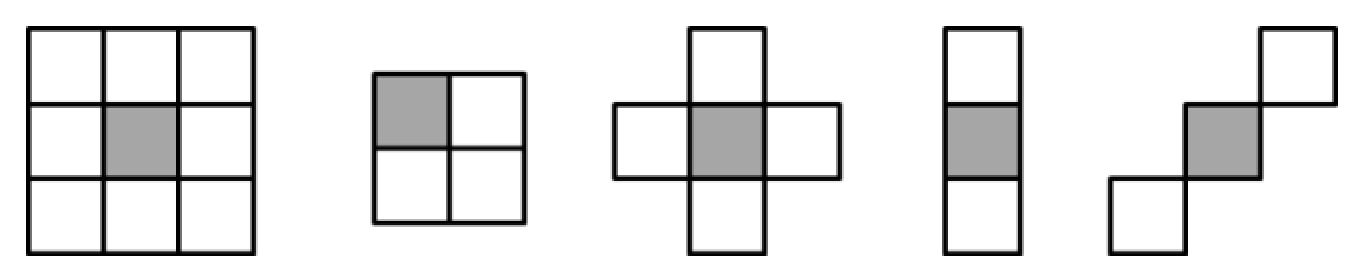
\includegraphics[scale=0.5]{../fig/structelem.png}
\end{center}
Morphologische Operatoren dienen dazu die Form von Objekten in definierte Weise zu verändern. 
Dies sind typisch:
\begin{itemize}
	\item Löschen kleiner Objekte (z.B. Pixelrauschen) 
	\item Schliessen von Löchern in Objekten
	\item Zusammenfassen von räumlich nahen Objekten
	\item Löschen aller Pixel im Inneren eines Objektes
	\item Reduzieren eines Objektes auf das Skelett
\end{itemize}

\subsubsection{Dilatation}
Bei der Dilatation wird das Strukturelement über das Bild geschoben.
Dabei werden alle Referenzpunkte des Strukturelementes markiert, bei denen eine nicht verschwindende Schnittmenge mit dem Objekt auftritt.
\begin{center}
	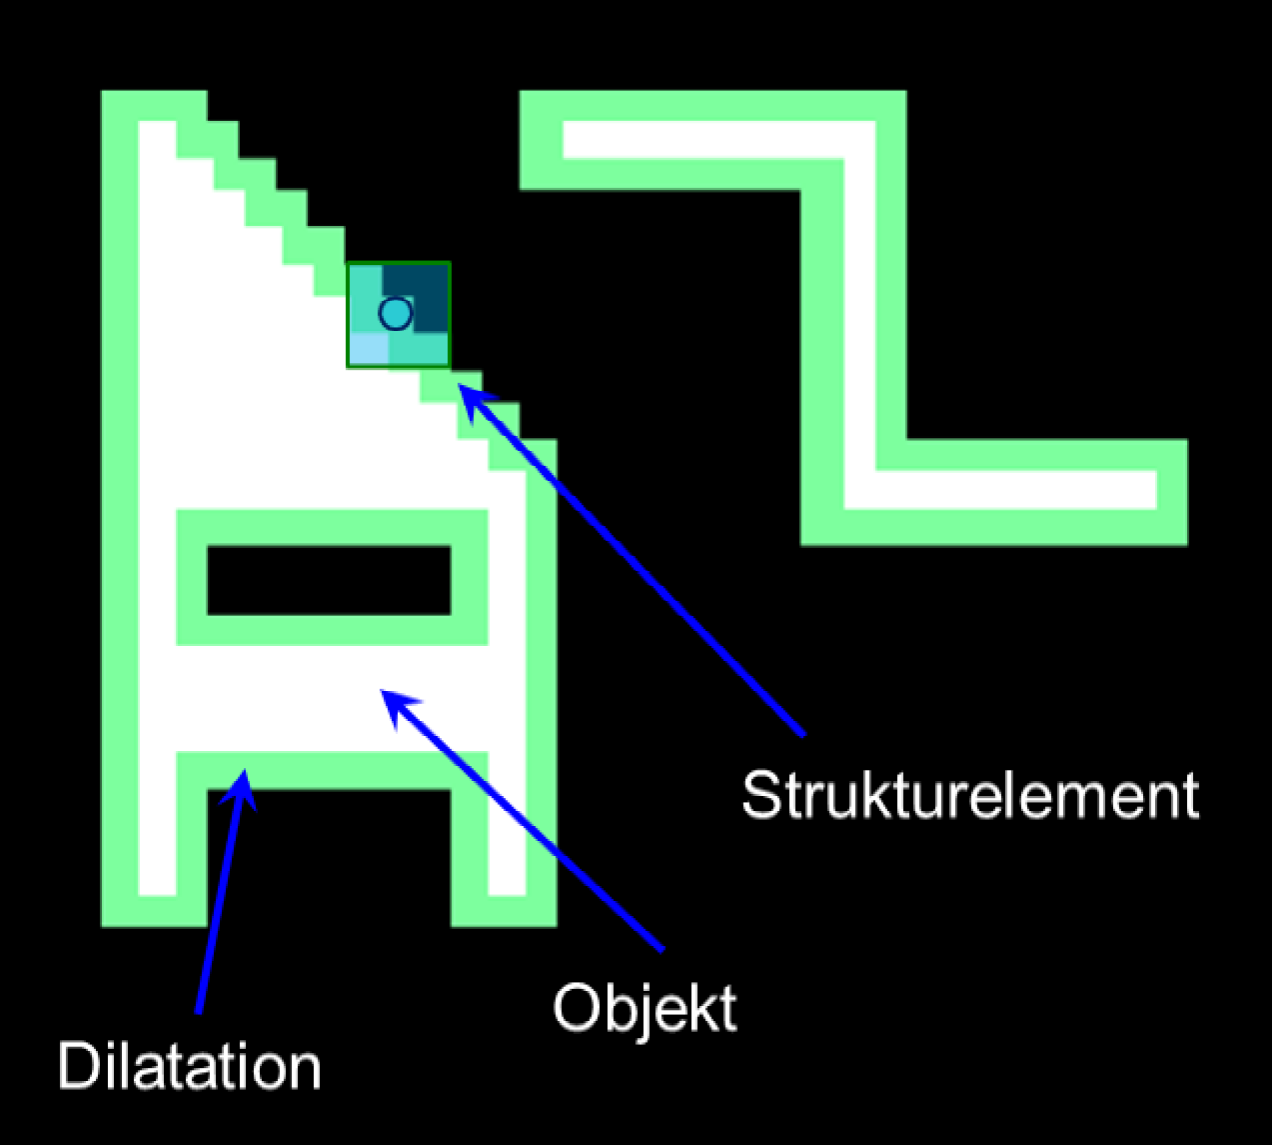
\includegraphics[scale=0.5]{../fig/dilatation.png}
\end{center}
Mathematische Beschreibung:
\[
	I \otimes h = \left\lbrace (m,n) | (\hat{h})_{m,n} \cap I \neq \{\} \right\rbrace
\]

\subsubsection{Erosion}
Bei der Dilatation wird das Strukturelement über das Bild geschoben.
Dabei werden alle Referenzpunkte des Strukturelementes markiert, bei denen das Strukturelement ganz in dem Objekt enthalten ist.
\begin{center}
	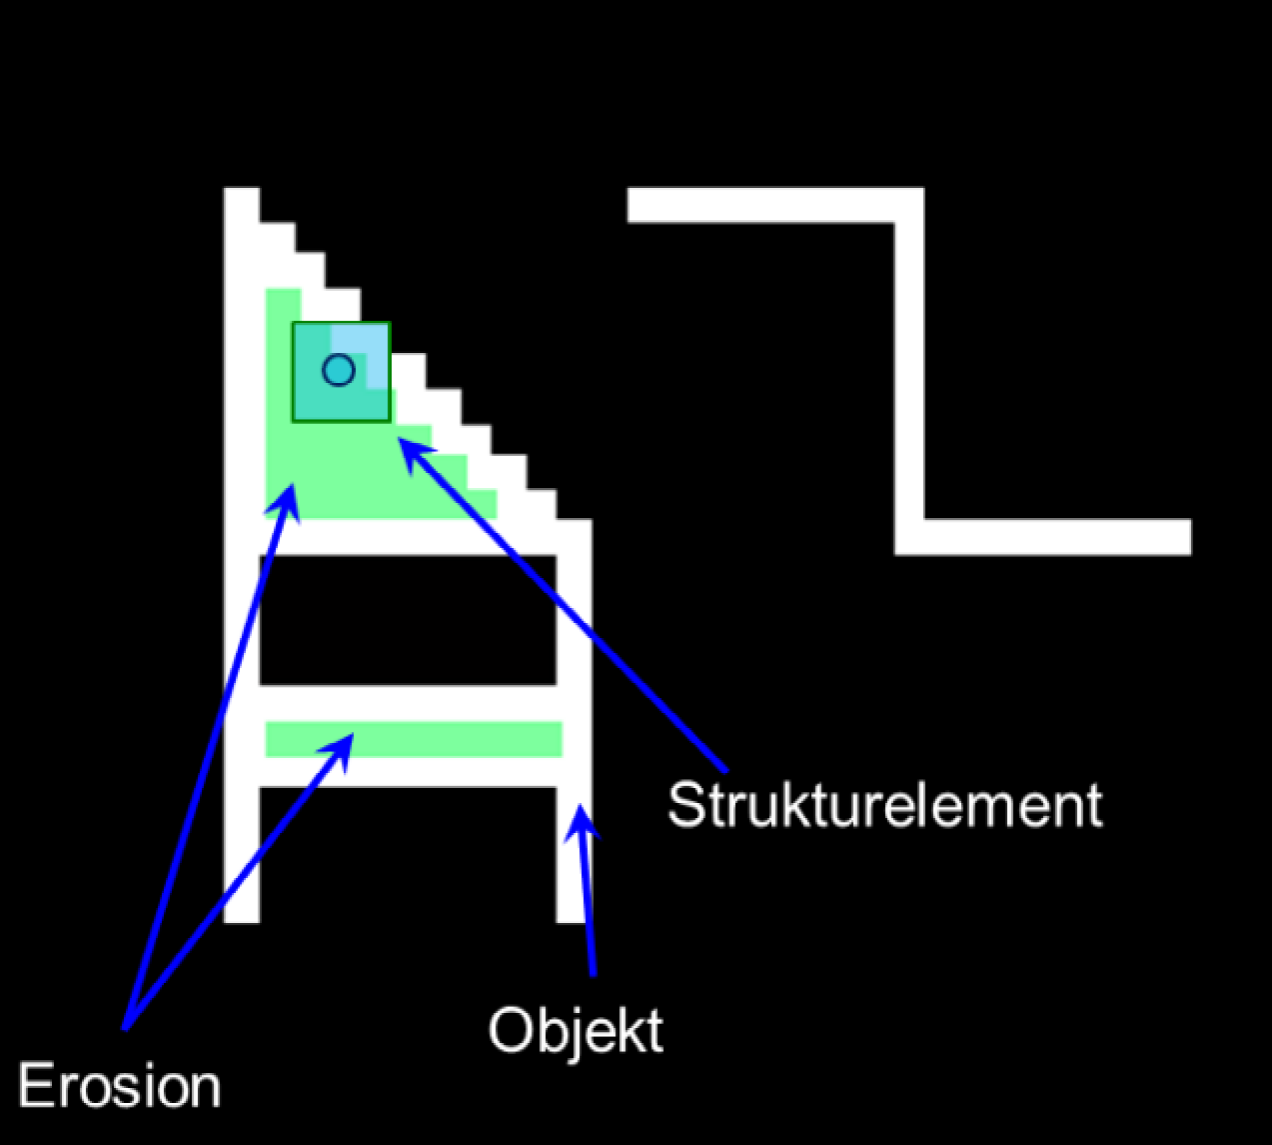
\includegraphics[scale=0.5]{../fig/erosion.png}
\end{center}
Mathematische Beschreibung:
\[
	I - h = \left\lbrace (m,n) | (h)_{m,n} \subset I \right\rbrace
\]

\subsubsection{Schliessung \& Öffnung}
Wen die Dilatation und Erosion kombiniert werden, entstehen weitere wichtige Operatoren.
Wird zuerst eine Dilatation dann eine Erosion ausgeführt, so entsteht eine Schliessung.
Umgekehrt eine Öffnung.
Mit der Schliessung können kleine Lücken geschlossen werden.
Die Öffnung kann Bildrauschen entfernen, da kleine Teile entfernt werden.\\
\\
Schliessung:
\[
	I \bullet h = (I \otimes h) - h
\]
~\\
Öffnung:
\[
	I \circ h = (I - h) \otimes h
\]
~\\\\
Lösung in MATLAB:
\lstset{language=Matlab}
\lstinputlisting[firstline=1,caption=]{../Matlab/morphologie.m}
~\\

\subsubsection{Hit- und Miss-Operation}
Bei dieser Operation wird nicht nur geschaut, ob das Strukturelement in einem Objekt enthalten ist, sondern ob die Nachbarschaft eine vorgegebene Struktur hat.
\begin{center}
	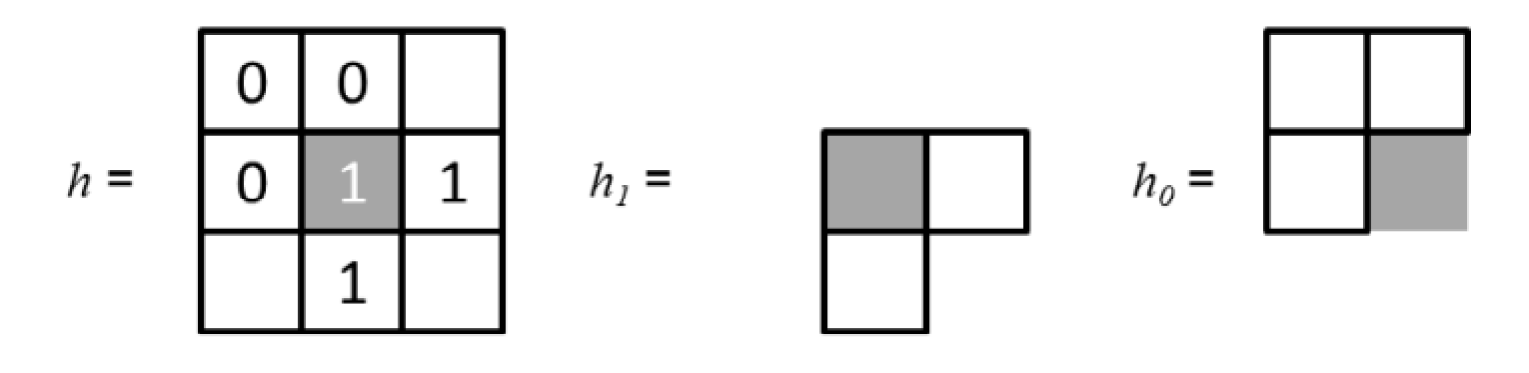
\includegraphics[scale=0.5]{../fig/hitmiss.png}
\end{center}
\begin{footnotesize}
	$0$: Das Pixel muss den Wert 0 haben\\
	$1$: Das Pixel muss den Wert 255 (bzw. 1) haben\\
	,,'': Der Wert des Pixels wird nicht in Betracht gezogen.\\
\end{footnotesize}
\\
Die mathematische Beschreibung:
\[
	I \pm h = (I - h_1) \cap (I^C - h_0)
\]
\begin{footnotesize}
	$I^C$: Das Komplement aller Pixel ungleich Null vom Bild $I$\\
\end{footnotesize}
\\
Hit- und Miss-Operation wird meist in Verbindung mit Verdünnungs- und Verdickungs-Operationen verwendet:
\[
	\text{thin}(I,h) = I \cap (I \pm h)^C
\]
		
% coding:utf-8

%----------------------------------------
%FOSAEBV, a LaTeX-Code for a summary of realtime image processing
%Copyright (C) 2013, Mario Felder

%This program is free software; you can redistribute it and/or
%modify it under the terms of the GNU General Public License
%as published by the Free Software Foundation; either version 2
%of the License, or (at your option) any later version.

%This program is distributed in the hope that it will be useful,
%but WITHOUT ANY WARRANTY; without even the implied warranty of
%MERCHANTABILITY or FITNESS FOR A PARTICULAR PURPOSE.  See the
%GNU General Public License for more details.
%----------------------------------------

\chapter{Fourier-Transformation}

\section{1D Fourier-Transformation}
Die Fourier Transformationen dient dazu, für eine Funktion $h(x)$ im Ortsraum das zugehörige Frequenzspektrum im Ortsfrequenzraum $\hat{h}(f)$  zu bestimmen.
Dabei gibt es grundsätzlich vier mögliche Anwendungsfälle und zugehörige Formulierungen der Fourier Transformation (FT):

\paragraph{Kontinuierliche FT einer aperiodischen Funktion $h(x)$:}
\[
	\hat{h}(f) = \int_{-\infty}^{\infty} h(x) \cdot \e^{-\im \cdot 2\pi \cdot f \cdot x}\di x \qquad
	h(f) = \int_{-\infty}^{\infty} \hat{h}(x) \cdot \e^{\im \cdot 2\pi \cdot f \cdot x}\di f
\]

\paragraph{Kontinuierliche FT einer $X_0$-periodischen Funktion $h(x)$:}
\[
	\hat{h}[n] = \frac{1}{X_0}\int_{0}^{X_0} h(x) \cdot \e^{-\im \cdot 2\pi \cdot f_0 \cdot x}\di x \qquad
	h(f) = \sum_{n=-\infty}^{\infty} \hat{h}[n] \cdot \e^{\im \cdot 2\pi \cdot n \cdot f_0 \cdot x}
\]
\begin{footnotesize}
	$f_0 = \frac{1}{X_0}$\\
\end{footnotesize}
~\\
Im Falle einer periodischen Funktion besteht das Frequenzspektrum nur aus diskreten Werten an den Frequenzen $f_n = n \cdot f_0$.

\paragraph{Diskrete FT einer aperiodischen Funktion für äquidistante Abtastpunkte $h_n = h(n\cdot x_s)$:}
\[
	\hat{h}(f) = \sum_{n = -\infty}^{\infty} h[n] \cdot \e^{-\im \cdot 2\pi \cdot f \cdot n \cdot x_s} \qquad
	h[n] = \frac{1}{f_s}\int_{0}^{f_s} \hat{h}(f) \cdot \e^{\im \cdot 2\pi \cdot n \cdot x_s \cdot f}\di f
\]
\begin{footnotesize}
	$f_s = \frac{1}{x_s}$\\
\end{footnotesize}
~\\
Bei Abtastung eines Signals mit dem Intervall $x_s$ entsteht ein periodisches Frequenzspektrum der Periode $f_s$.

\paragraph{Diskrete FT einer $X_0$-periodischer Funktion für äquidistante Abtastpunkte $h_n = h(n\cdot x_s)$:}
\[
	\hat{h}[k] = \sum_{n=0}^{N-1} h[n] \cdot \e^{-\im \cdot 2\pi \cdot \frac{k \cdot n}{N}} \qquad
	h[n] = \frac{1}{N} \sum_{k=0}^{N-1} \hat{h}[k] \cdot \e^{\im \cdot 2\pi \cdot \frac{k \cdot n}{N}}
\]
\begin{footnotesize}
	$x_s =\frac{X_0}{N}$\\
\end{footnotesize}
~\\
Wird ein periodisches Signal mit $n \cdot x_0$ Intervallpunkten abgetastet, so hat die FT ein ebenfalls diskretes und periodisches Frequenzspektrum der Periode $f_s = \frac{1}{x_s} = \frac{N}{X_0}$.
\\

\paragraph{Rechenregeln\\}
\begin{tabular}{ll}
	Linearität: & $\mathcal{F}\{\lambda \cdot h(x)\} = \lambda \cdot \mathcal{F}\{h(x)\}$ \\
	 & $\mathcal{F}\{h(x) + g(x)\} = \mathcal{F}\{h(x)\} + \mathcal{F}\{g(x)\}$\\
	Verschiebung: & $\mathcal{F}\{h(x+x_0)\} = \e^{\im \cdot 2\pi \cdot f \cdot x_0} \cdot \mathcal{F}\{h(x)\}$\\
	Faltungssatz: & $\mathcal{F}\{h(x) \otimes g(x)\} = \mathcal{F}\{h(x)\} \cdot \mathcal{F}\{g(x)\}$\\
\end{tabular}

\section{Diskrete 2D Fourier-Transformation}
Bei Annahme dass die Funktion in $x$-Richtung $X_0$-periodisch und in $y$-Richtung $Y_0$-periodisch ist ($X_0 = N \cdot x_s$, $Y_0 = M \cdot y_s$), so ist die 2D DFT folgendermassen definiert:
\[\begin{aligned}
	\hat{h}[l,k] &= \sum_{m=0}^{M-1} \sum_{n=0}^{N-1} h[m,n] \cdot \e^{-\im \cdot 2\pi \cdot \left[\frac{l \cdot m}{M} + \frac{k \cdot n}{N}\right]}
	\\
	h[m,n] &= \frac{1}{M \cdot N} \sum_{l=0}^{M-1} \sum_{k=0}^{N-1} \hat{h}[l,k] \cdot \e^{\im \cdot 2\pi \cdot \left[\frac{l \cdot m}{M} + \frac{k \cdot n}{N}\right]}
\end{aligned}\]
~\\\\
Lösung in MATLAB:
\lstset{language=Matlab}
\lstinputlisting[firstline=1,caption=]{../Matlab/dft.m}
~\\

\section{Periodische Strukturen}
Periodische Strukturen führen auch zu einem periodischen Frequenzspektrum.
Wenn das Bild jedoch nicht über den Bildrand hinaus periodisch ist, treten Fehler in der DFT auf.
Dies kann korrigiert werden, indem eine Fensterfunktion angewendet wird, welche zum Rand des Bildes stetig nach Null abfällt.
~\\\\
Lösung in MATLAB:
\lstset{language=Matlab}
\lstinputlisting[firstline=1,caption=]{../Matlab/hann.m}
~\\

\section{Unterdrückung periodischer Störungen}
Periodische Störungen haben auch eine periodische Auswirkung im Frequenzspektrum.
Durch einen Nochtfilter können diese selektiv ausgeblendet werden. So kann ein Grossteil des Rauschens eliminiert werden.
~\\\\
Lösung in MATLAB:
\lstset{language=Matlab}
\lstinputlisting[firstline=1,caption=]{../Matlab/notch.m}
~\\

\section{Deconvolution}
Ein Bild, welches durch einen Filter unscharf gezeichnet wurde, kann durch Deconvolution wieder hergestellt werden. Dabei wird der Faltungssatz angewendet.
~\\\\
Lösung in MATLAB:
\lstset{language=Matlab}
\lstinputlisting[firstline=1,caption=]{../Matlab/deconvolution.m}
~\\
		
% coding:utf-8

%----------------------------------------
%FOSAEBV, a LaTeX-Code for a summary of realtime image processing
%Copyright (C) 2013, Mario Felder

%This program is free software; you can redistribute it and/or
%modify it under the terms of the GNU General Public License
%as published by the Free Software Foundation; either version 2
%of the License, or (at your option) any later version.

%This program is distributed in the hope that it will be useful,
%but WITHOUT ANY WARRANTY; without even the implied warranty of
%MERCHANTABILITY or FITNESS FOR A PARTICULAR PURPOSE.  See the
%GNU General Public License for more details.
%----------------------------------------

\chapter{Segmentierung und Merkmalsextraktion}

\section{Automatisierte Schwellwertbestimmung}
Das Verfahren von Otsu basiert darauf, dass alle Grauwerte in zwei Klassen eingeteilt werden ($C_0 = \{0,1,...,K\}$ und $C_1=\{K+1,...,255\}$). 
$K$ stellt den zu optimierenden Schwellwert dar.
Es wird angenommen, dass das Bild eine bimodale Grauwertverteilung hat.
Das Bild zerfällt in zwei Klassen mit relativ homogenen Grauwerten.
Der Schwellwert $K$ wird so optimiert, dass die Varianzen innerhalb der Klassen möglichst klein sind.\\
\\
Wahrscheinlichkeit für Auftreten von Klasse $C_0$ bzw. $C_1$:
\[
	\omega_0 = \sum_{g=0}^{K}p_I(g) \qquad 
	\omega_1 = \sum_{g=K+1}^{255}p_I(g)
\]
Mittelwert der Grauwerte von Klasse $C_0$ bzw. $C_1$:
\[
	\mu_0 = \frac{1}{\omega_0} \sum_{g=0}^{K} p_I(g) \cdot g \qquad
	\mu_1 = \frac{1}{\omega_1} \sum_{g=K+1}^{255} p_I(g) \cdot g
\]
Varianz der Grauwerte von Klasse $C_0$ bzw. $C_1$:
\[
	{\sigma_0}^2 = \frac{1}{\omega_0} \sum_{g=0}^{K} p_I(g) \cdot (g - \mu_0)^2 \qquad
	{\sigma_1}^2 = \frac{1}{\omega_1} \sum_{g=K+1}^{255} p_I(g) \cdot (g - \mu_1)^2
\]
Intra-Klassen Varianz:
\[
	{\sigma_W}^2 = \omega_0 \cdot {\sigma_0}^2 + \omega_1 \cdot {\sigma_1}^2
\]
Optimaler Schwellwert nach Otsu:
\[
	K_{opt} = \arg \min \{\sigma_w\}
\]
~\\\\
Dargestellt mit der Inter-Klassen Varianz:
\[
	{\sigma_B}^2 = \omega_0 \cdot (\mu_0 - \mu_T)^2 + \omega_1 \cdot (\mu_1 - \mu_T)^2
\]
Globaler Mittelwert aller Grauwerte:
\[
	\mu_T = \sum_{g=0}^{255}p_I(g) \cdot g
\]
~\\
Da die Summe der Intra-Klassen Varianz und der Inter-Klassen Vrianz konstant ist, kann anstatt $\sigma_W$ minimiert, $\sigma_B$ maximiert werden.
Dies hat den Vorteil, dass die Inter-Klassen Varianz einfach berechnet werden kann.
\[\begin{aligned}
	K_{opt} &= \arg\max\{\sigma_B\}\\
	{\sigma_B}^2 &= \omega_0 \cdot \omega_1 \cdot (\mu_0 - \mu_1)^2
\end{aligned}\]
~\\\\
Lösung in MATLAB:
\lstset{language=Matlab}
\lstinputlisting[firstline=1,caption=]{./Matlab/otsu.m}
~\\
Lösung in MATLAB:
\lstset{language=Matlab}
\lstinputlisting[firstline=1,caption=]{./Matlab/OwnOtsu.m}
~\\

\section{Beschreibung der ROIs}
Für die Verarbeitung müssen ROIs (Region of Intress) beschreiben werden, um in einem weiteren Schritt deren Merkmale zu extrahieren.

\subsection{Region Labeling}
Beim Region Labeling wird das Bild zeilenweise durch iteriert.
Dabei wird jedem Pixel ungleich Null ein Label zugeordnet.
Wenn ein Nachbarpixel (Achter-Nachbarschaftsrelation) bereits ein Label enthält, erhält das aktuelle Pixel das gleiche Label, sonst ein neues.
Am schluss wird noch überprüft, ob die Label Werte der Nachbarpixel unterschiedlich sind.
Falls dies der Fall ist, so wird in einer Lookup Tabelle festgehalten, 
dass die entsprechenden Label Werte zu einem Objekt gehören.
In einem weiteren Durchgang werden die Labelwerte einer Gruppe durch den kleinsten Wert der Gruppe ersetzt.
\begin{center}
	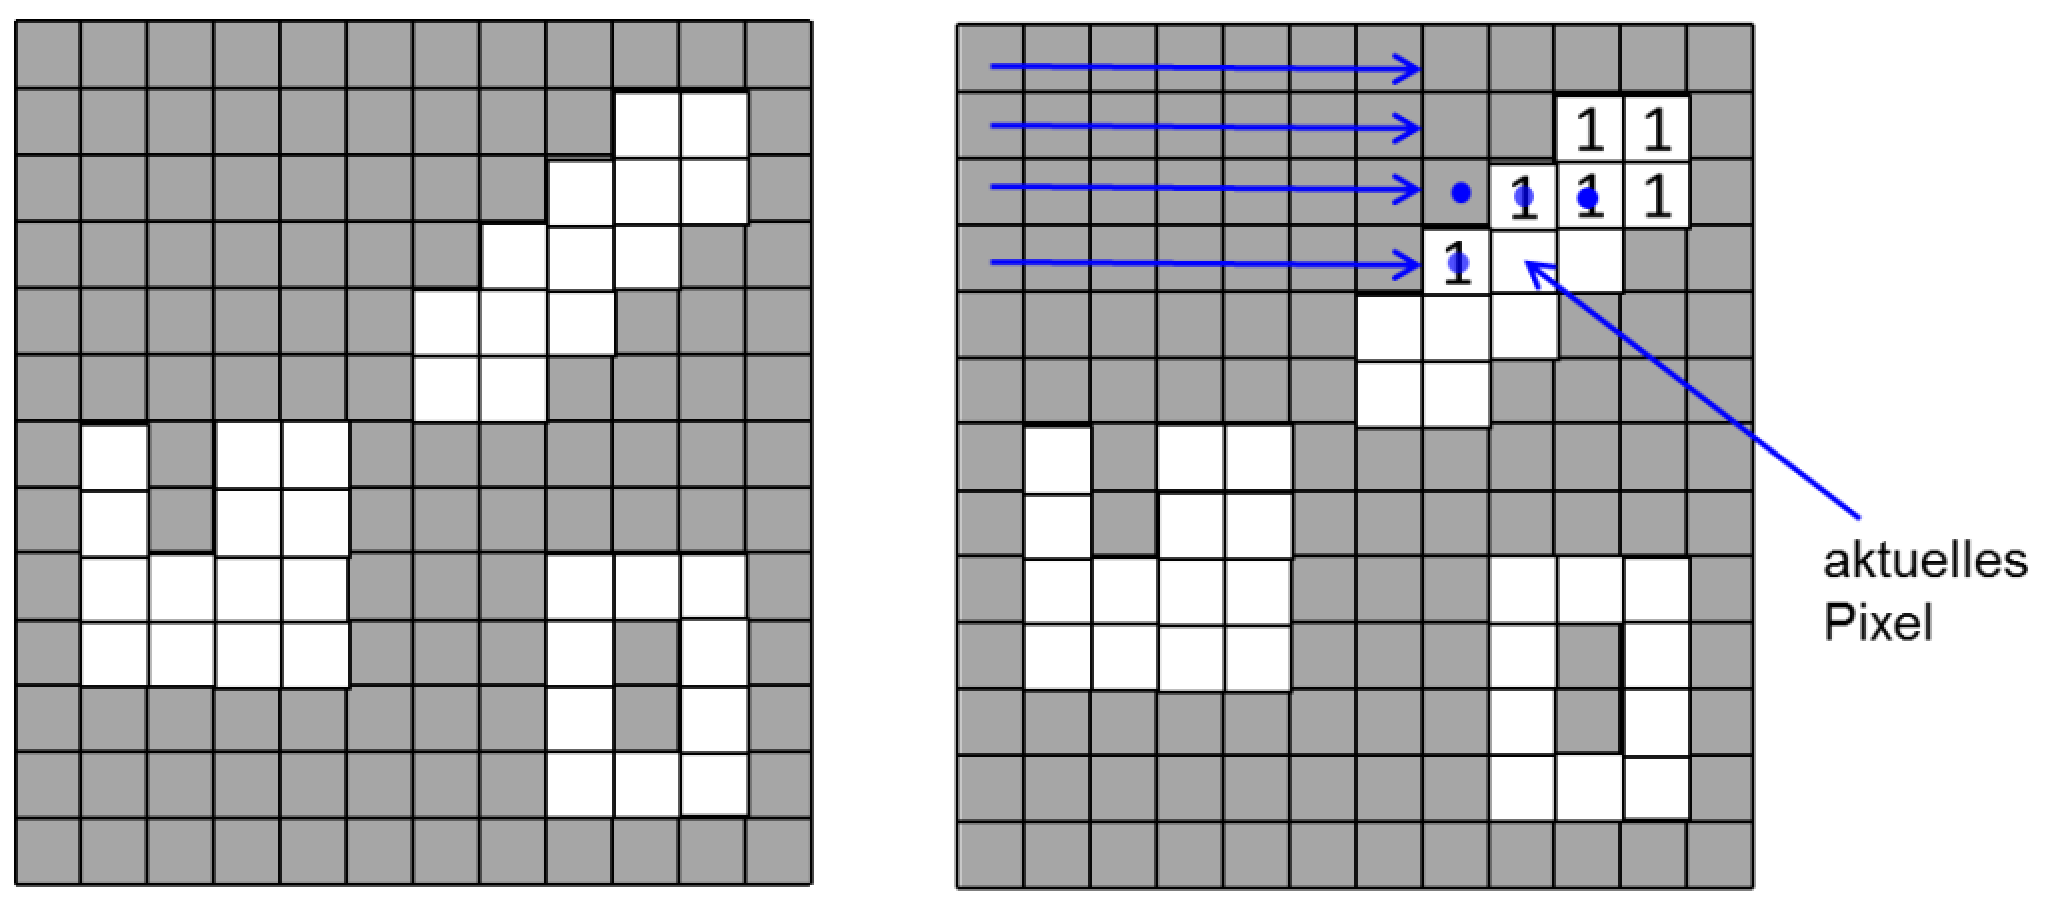
\includegraphics[scale=.5]{./images/labeling.png}
\end{center}
\begin{center}
	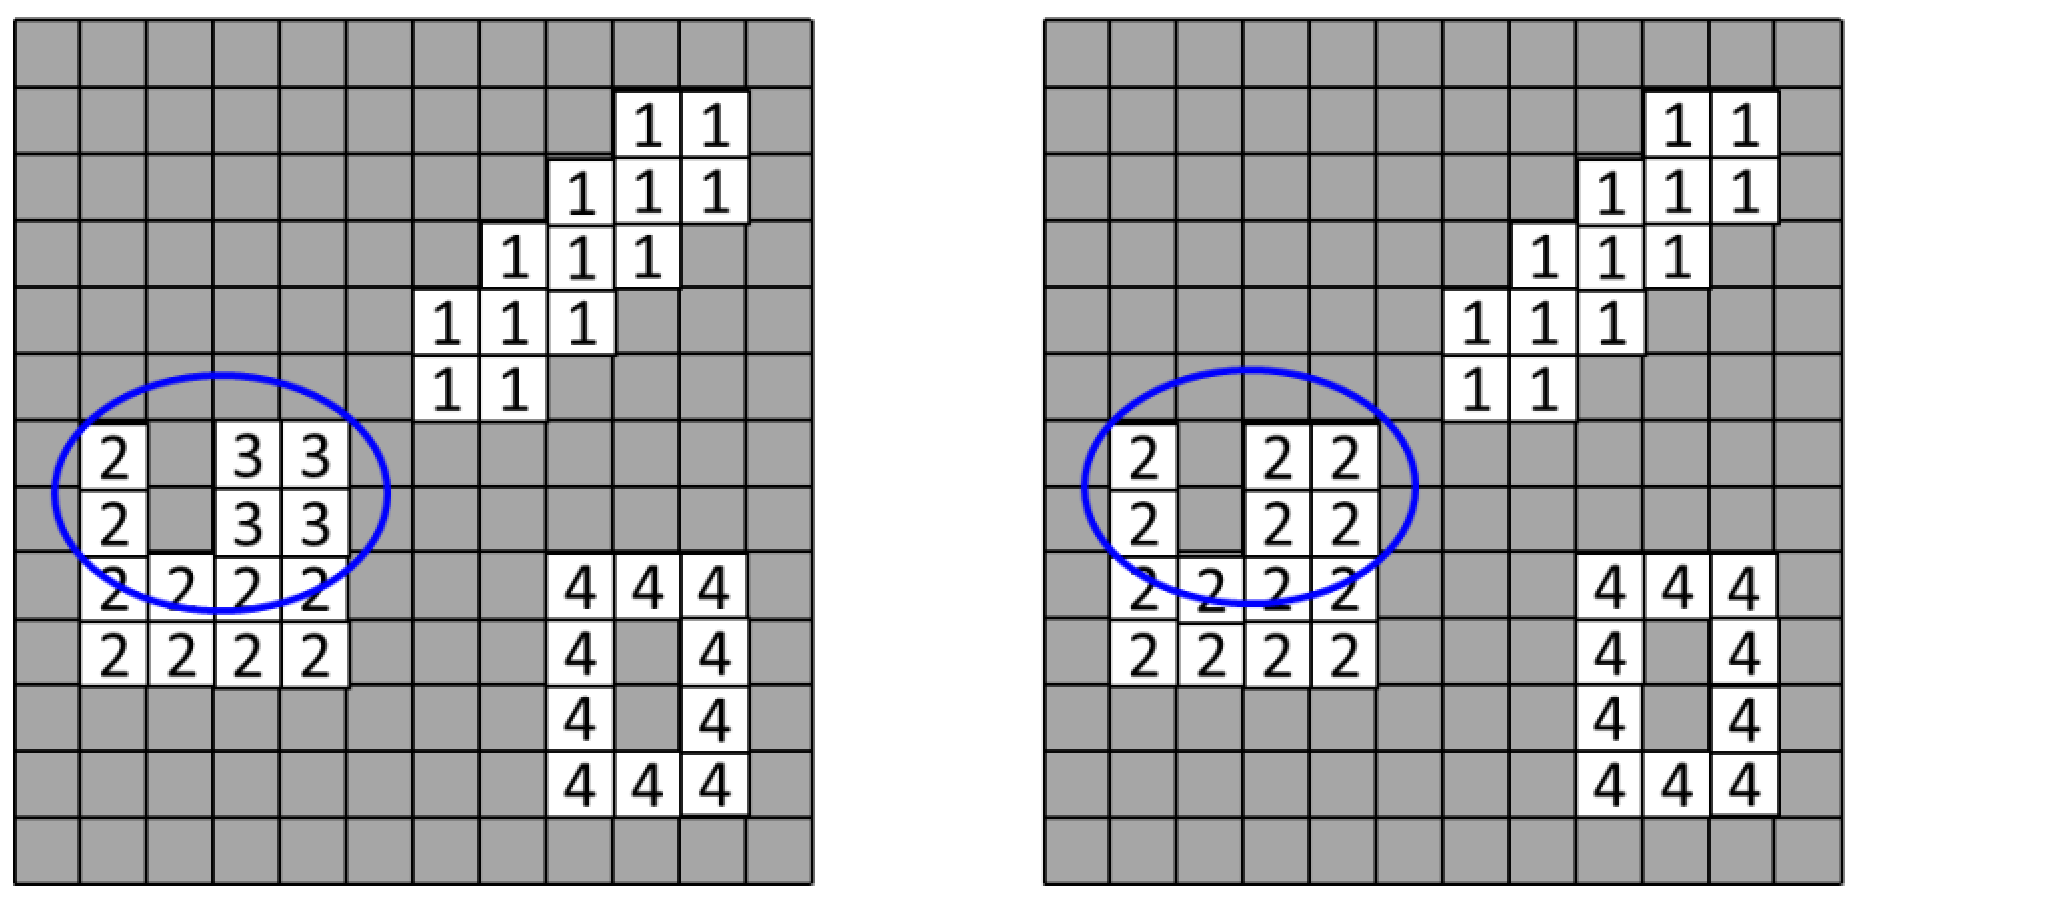
\includegraphics[scale=.5]{./images/labeling2.png}
\end{center}

\subsection{Kettencode}
Da das Region Labeling häufig einen relativ grossen Speicherbedarft hat, werden in der Regel Kettencodes zur Beschreibung von ROIs verwendet.\\
Die Idee ist, die Randpixel einer ROI, 
ausgehen von einem definierten Startpunkt, 
in sukzessiver Folge nur durch die jeweilige Schrittrichtung vom letzten zum aktuellen Randpixel zu definieren.
\begin{center}
	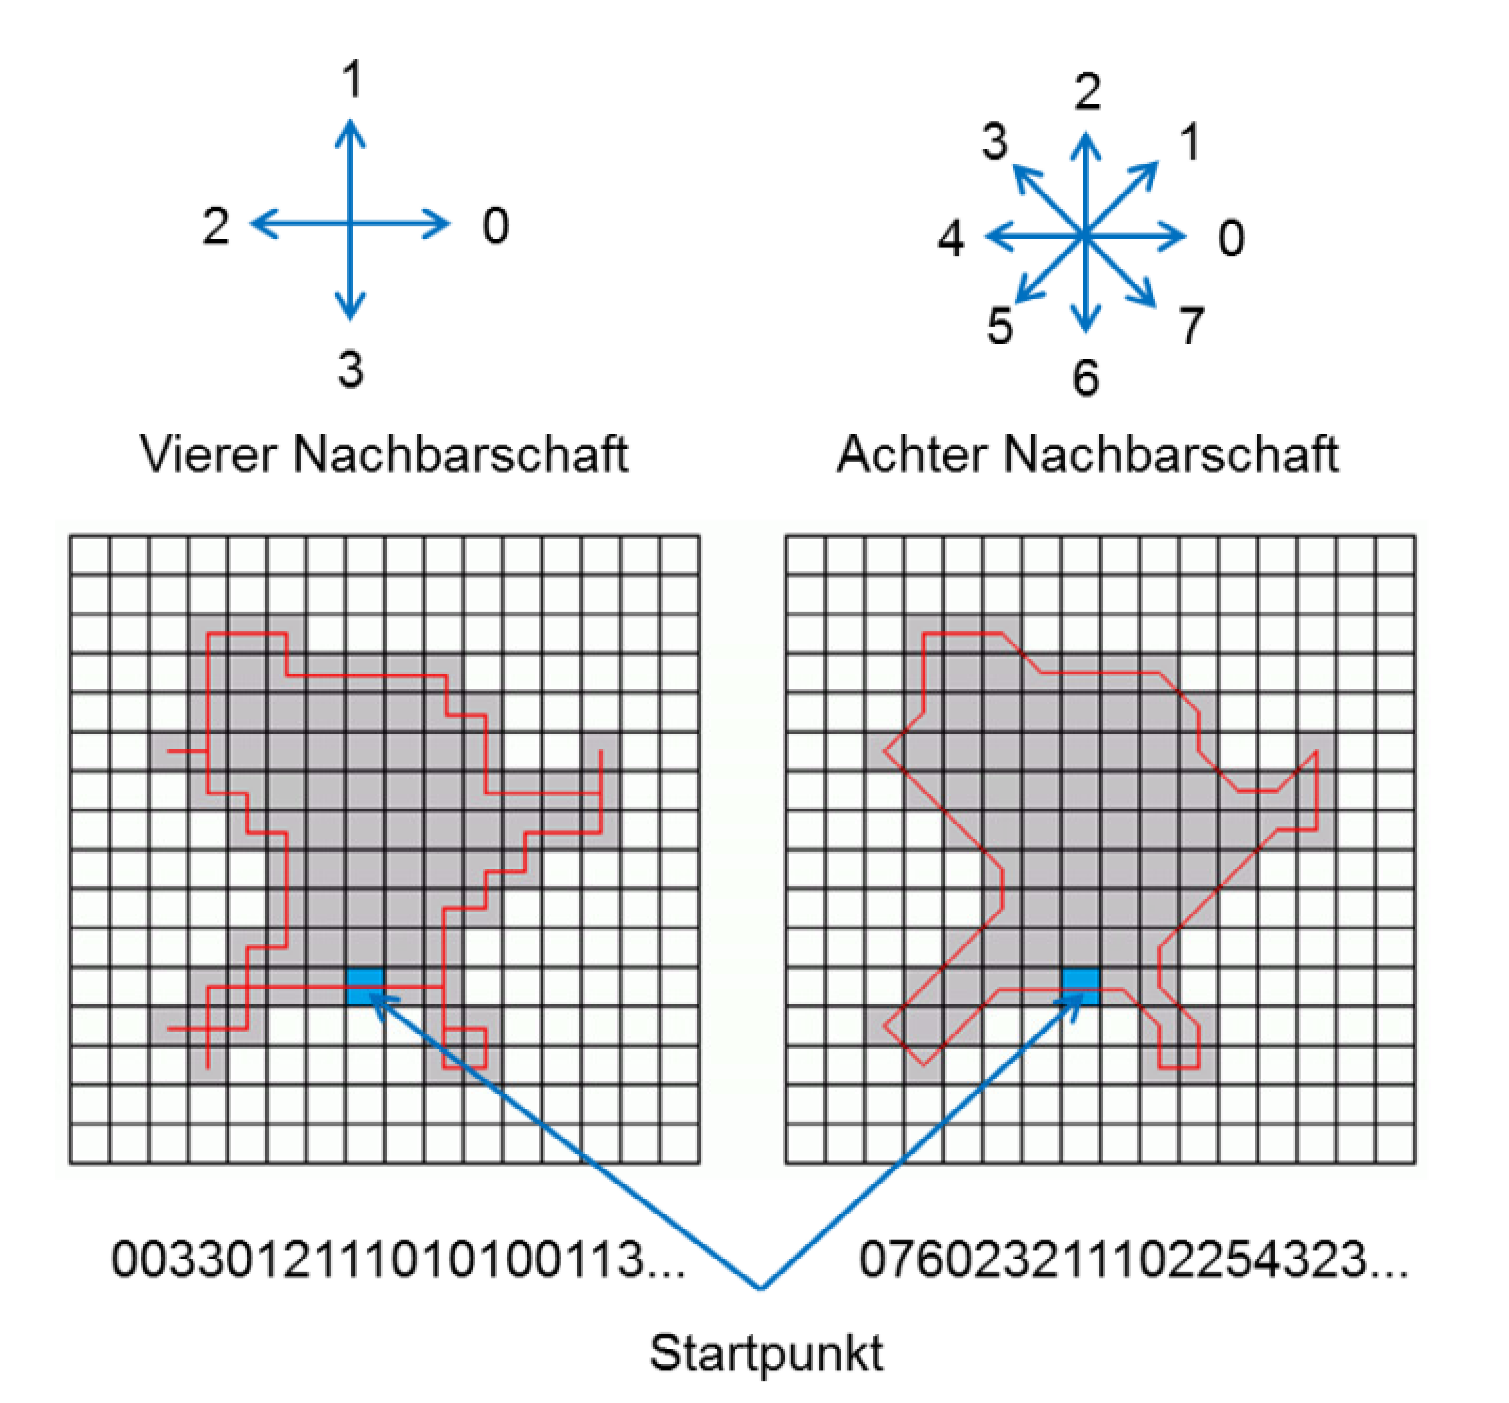
\includegraphics[scale=.5]{./images/kettencode.png}
\end{center}

\section{Merkmalsextraktion}
Basierend auf der Beschreibung der ROIs mittels Region Labels oder Kettencodes können nun einfach verschiedene ROI Merkmale extrahiert werden.\\
\\
\paragraph{Fläche der ROI:}
\[
	A = \sum_{I_{mn} \in ROI}1
\]
Berechnung anhand von Kettencodes mit dem Crack Code (stellt die Trennlinie zwischen Vorder- und Hintergrund dar):
\[
	A = -\oint_{Rand}y(x)\di x = \sum_{I_{mn} \in \{2-Seg.\}}m - \sum_{I_{mn} \in \{0-Seg.\}}m 
\]
~\\\\
\paragraph{Massnemittelpunkt der ROI:}
\[
	x_s = \frac{1}{A} \sum_{I_{mn}\in ROI}n \qquad y_s = \frac{1}{A} \sum_{I_{mn}\in ROI}m
\]
~\\\\
\paragraph{Umfang der ROI:\\}
Im Falles einer Crack Code basierten Beschreibung der ROIs ist der Umfang einfach durch die Anzahl der Segmente des Codes geben.\\
\\
\paragraph{Orientierung der ROI:\\}
Die Orientierung einer ROI ist definiert als der Winkel zwischen der x-Achse und der längeren der beiden Halbachsen der ROI.
Dabei sind die Halbachsen bestimmt durch die Eigenvektoren der symmetrischen Matrix bestehend aus den zweiten Momenten $M_{xy}$  der ROI:
\begin{scriptsize}\[\begin{aligned}
	M &= \left[\begin{matrix}
	 M_{xx} & M_{xy}\\
	 M_{xy} & M_{yy}\\
	\end{matrix}\right]\\\\
	M_{xx} = \frac{1}{A}\sum_{I_{mn}\in ROI}n^2-{x_s}^2& \qquad
	M_{yy} = \frac{1}{A}\sum_{I_{mn}\in ROI}m^2-{y_s}^2 \\
	M_{xy} &= \frac{1}{A}\sum_{I_{mn}\in ROI}n \cdot m-x_s \cdot y_s
\end{aligned}\]\end{scriptsize}
~\\\\
\paragraph{Bounding Box\\}
Dies ist das kleinste Rechteck, das die ROI noch ganz umschliesst. 
Es ist vor allem nützlich, um schnell Tests bezüglich von Einflussregionen durchzuführen.

~\\\\
Lösung in MATLAB:
\lstset{language=Matlab}
\lstinputlisting[firstline=1,caption=]{./Matlab/MerkmalsExtraktion.m}
~\\		
% coding:utf-8

%----------------------------------------
%FOSAEBV, a LaTeX-Code for a summary of realtime image processing
%Copyright (C) 2013, Mario Felder

%This program is free software; you can redistribute it and/or
%modify it under the terms of the GNU General Public License
%as published by the Free Software Foundation; either version 2
%of the License, or (at your option) any later version.

%This program is distributed in the hope that it will be useful,
%but WITHOUT ANY WARRANTY; without even the implied warranty of
%MERCHANTABILITY or FITNESS FOR A PARTICULAR PURPOSE.  See the
%GNU General Public License for more details.
%----------------------------------------

\chapter{Linien-Segmentierung und Merkmalsextraktion}
%% coding:utf-8

%----------------------------------------
%FOSAEBV, a LaTeX-Code for a summary of realtime image processing
%Copyright (C) 2013, Mario Felder

%This program is free software; you can redistribute it and/or
%modify it under the terms of the GNU General Public License
%as published by the Free Software Foundation; either version 2
%of the License, or (at your option) any later version.

%This program is distributed in the hope that it will be useful,
%but WITHOUT ANY WARRANTY; without even the implied warranty of
%MERCHANTABILITY or FITNESS FOR A PARTICULAR PURPOSE.  See the
%GNU General Public License for more details.
%----------------------------------------

\chapter{Farbe}
%% coding:utf-8

%----------------------------------------
%FOSAEBV, a LaTeX-Code for a summary of realtime image processing
%Copyright (C) 2013, Mario Felder

%This program is free software; you can redistribute it and/or
%modify it under the terms of the GNU General Public License
%as published by the Free Software Foundation; either version 2
%of the License, or (at your option) any later version.

%This program is distributed in the hope that it will be useful,
%but WITHOUT ANY WARRANTY; without even the implied warranty of
%MERCHANTABILITY or FITNESS FOR A PARTICULAR PURPOSE.  See the
%GNU General Public License for more details.
%----------------------------------------

\chapter{Anwendungen}

\end{document}

